\ifdefined\inMainDoc\else
\documentclass[12pt,a4paper]{article}
% ================================================================
%  PRÉAMBULE COMMUN - ANNALES CORRIGÉES
%  Université de Kara - FaST - Licence Fondamentale MPC
%  Design optimisé impression noir et blanc
% ================================================================

% -- ENCODAGE & LANGUE --
\usepackage[utf8]{inputenc}
\usepackage[T1]{fontenc}
\usepackage[french]{babel}
\usepackage{lmodern}
\usepackage{microtype}

% -- MISE EN PAGE --
\usepackage[a4paper, top=2.8cm, bottom=2.5cm, left=2.5cm, right=2.5cm, headheight=14pt]{geometry}
\usepackage{setspace}
\setstretch{1.2}
\usepackage{parskip}
\setlength{\parindent}{1.2em}
\setlength{\parskip}{4pt}

% -- MATHS --
\usepackage{amsmath, amssymb, mathtools, amsthm}
\usepackage{mathrsfs}
\usepackage{dsfont}
\usepackage{bm}
\usepackage{cancel}
\usepackage{textcomp}
% Définition de \oiint (intégrale de surface fermée) sans package supplémentaire
\newcommand{\oiint}{\mathop{\iint\!\!\!\!\!\!\!\bigcirc}\limits}

% -- PHYSIQUE & CHIMIE --
\usepackage{physics}
\usepackage{siunitx}
% Lorsque physics est chargé, siunitx omet \qty. On le restaure ici :
\AtBeginDocument{\RenewCommandCopy\qty\SI}
\sisetup{locale = FR, detect-all, output-decimal-marker={,}}
% Commande de substitution pour les unités posant problème avec pdflatex
% (ohm, degreeCelsius, micro, angstrom, percent utilisent des caractères non-ASCII)
\newcommand{\qtyohm}[1]{\ensuremath{\num{#1}\,\Omega}}
\newcommand{\qtydegc}[1]{\ensuremath{\num{#1}\,{}^\circ\text{C}}}
\newcommand{\qtyangstrom}[1]{\ensuremath{\num{#1}\,\text{\AA}}}
\newcommand{\qtypercent}[1]{\ensuremath{\num{#1}\,\%}}
\newcommand{\qtyum}[1]{\ensuremath{\num{#1}\,\mu\text{m}}}
\usepackage[version=4]{mhchem}

% -- GRAPHISMES --
\usepackage{graphicx}
\usepackage{float}
\usepackage{caption}
\usepackage{subcaption}
\usepackage{wrapfig}
\usepackage{tikz}
\usetikzlibrary{calc, arrows.meta, patterns, shapes.geometric}
\usepackage{pgfplots}
\pgfplotsset{compat=1.18}

% -- TABLEAUX --
\usepackage{booktabs}
\usepackage{array}
\usepackage{tabularx}
\usepackage{multirow}

% -- LISTES --
\usepackage{enumitem}
\setlist[enumerate]{topsep=3pt, itemsep=2pt, parsep=0pt}
\setlist[itemize]{topsep=3pt, itemsep=2pt, parsep=0pt, label={.}}

% -- BOÎTES (noir et blanc) --
\usepackage{mdframed}
\usepackage{tcolorbox}
\tcbuselibrary{skins, breakable, theorems}

% Boîte EXERCICE : encadré avec filet épais, fond blanc
\newmdenv[
  linewidth=1.2pt,
  linecolor=black,
  roundcorner=3pt,
  skipabove=10pt,
  skipbelow=6pt,
  innertopmargin=8pt,
  innerbottommargin=8pt,
  innerleftmargin=10pt,
  innerrightmargin=10pt,
  backgroundcolor=white,
  frametitle={\bfseries\small Exercice},
  frametitlealignment=\raggedright,
  frametitleaboveskip=4pt,
  frametitlebelowskip=4pt,
]{boiteexercice}

% Boîte CORRIGÉ : fond gris très clair + filet fin
\newmdenv[
  linewidth=0.6pt,
  linecolor=black,
  leftline=true,
  rightline=false,
  topline=false,
  bottomline=false,
  linecolor=black,
  innerleftmargin=12pt,
  innerrightmargin=8pt,
  innertopmargin=6pt,
  innerbottommargin=6pt,
  backgroundcolor=gray!8,
  skipabove=4pt,
  skipbelow=8pt,
]{boitecorrige}

% Boîte RÉSUMÉ DE COURS : double encadré
\newmdenv[
  linewidth=0.8pt,
  linecolor=black,
  roundcorner=2pt,
  backgroundcolor=gray!12,
  innertopmargin=10pt,
  innerbottommargin=10pt,
  innerleftmargin=12pt,
  innerrightmargin=12pt,
  skipabove=12pt,
  skipbelow=8pt,
]{boiteresume}

% Boîte ATTENTION/REMARQUE : barre gauche épaisse
\newmdenv[
  leftline=true,
  rightline=false,
  topline=false,
  bottomline=false,
  linewidth=3pt,
  linecolor=black,
  backgroundcolor=gray!5,
  innerleftmargin=12pt,
  innerrightmargin=8pt,
  innertopmargin=5pt,
  innerbottommargin=5pt,
  skipabove=6pt,
  skipbelow=6pt,
]{boiteremarque}

% -- DIFFICULTÉ DES EXERCICES --
\newcommand{\facile}{$\star$}
\newcommand{\moyen}{$\star\!\star$}
\newcommand{\difficile}{$\star\!\star\!\star$}
\newcommand{\niveau}[1]{\hfill\textbf{#1}\hspace{2pt}}

% -- EN-TÊTES ET PIEDS DE PAGE --
\usepackage{fancyhdr}
\pagestyle{fancy}
\fancyhf{}
\renewcommand{\headrulewidth}{0.5pt}
\renewcommand{\footrulewidth}{0.3pt}

% -- HYPERLIENS --
\usepackage[hidelinks]{hyperref}
\hypersetup{
    colorlinks=false,
    pdftitle={Annale Corrigée - Licence MPC - Université de Kara}
}

% -- TITRES --
\usepackage{titlesec}
\titleformat{\section}{\Large\bfseries}{\thesection.}{0.8em}{}[\vspace{2pt}\hrule\vspace{4pt}]
\titleformat{\subsection}{\large\bfseries}{\thesubsection.}{0.7em}{}
\titleformat{\subsubsection}{\normalsize\bfseries}{\thesubsubsection.}{0.6em}{}

% -- THÉORÈMES --
\theoremstyle{definition}
\newtheorem{defn}{Définition}[section]
\newtheorem{prop}{Propriété}[section]
\newtheorem{thm}{Théorème}[section]
\newtheorem{corol}{Corollaire}[section]
\newtheorem{exemple}{Exemple}[section]

% -- COMMANDES MATHÉMATIQUES UTILES --
\newcommand{\vect}[1]{\overrightarrow{#1}}
\newcommand{\R}{\mathbb{R}}
\newcommand{\N}{\mathbb{N}}
\newcommand{\Z}{\mathbb{Z}}
\newcommand{\C}{\mathbb{C}}
\renewcommand{\d}{\mathrm{d}}
\newcommand{\deriv}[2]{\dfrac{\d #1}{\d #2}}
\newcommand{\dpart}[2]{\dfrac{\partial #1}{\partial #2}}
\newcommand{\rot}{\overrightarrow{\mathrm{rot}}\,}
\renewcommand{\div}{\mathrm{div}\,}
\renewcommand{\grad}{\overrightarrow{\mathrm{grad}}\,}
\newcommand{\e}{\mathrm{e}}
\newcommand{\ii}{\mathrm{i}}
\renewcommand{\Tr}{\mathrm{Tr}}

% Numérotation des équations par section
\numberwithin{equation}{section}

% -- RÉSULTATS ENCADRÉS --
\newcommand{\res}[1]{\[\boxed{#1}\]}

% -- REMARQUE INLINE --
\newcommand{\rmq}[1]{\begin{boiteremarque}\textbf{Remarque.} #1\end{boiteremarque}}

% -- MISE EN VALEUR DU RÉSULTAT FINAL --
\newcommand{\reponse}[1]{%
  \begin{center}
    \fbox{\begin{minipage}{0.92\textwidth}\centering #1\end{minipage}}
  \end{center}%
}


\lhead{\small\textit{Physique Nucléaire - Licence 3}}
\rhead{\small\textit{FaST, Université de Kara}}
\cfoot{\thepage}

\begin{document}
\fi

\begin{center}
  {\LARGE\bfseries PHYSIQUE NUCLÉAIRE ET RADIOACTIVITÉ}\\[0.3cm]
  {\normalsize Licence 3 - Physique}\\[0.1cm]
  \rule{0.7\textwidth}{0.8pt}
\end{center}

\section*{Résumé du cours}

\begin{boiteresume}

\textbf{1. Structure du noyau.} Un noyau ${}^A_Z$X contient $Z$ protons et $N = A-Z$ neutrons. La masse du noyau est inférieure à la somme des masses de ses constituants : c'est le défaut de masse $\Delta m = Zm_p + Nm_n - m_{noyau}$. L'énergie de liaison est $E_L = \Delta m\cdot c^2$.

\textbf{2. Loi de désintégration radioactive.} À chaque instant, un échantillon de $N$ noyaux radioactifs se désintègre à un taux proportionnel à $N$ :
\[
\frac{\d N}{\d t} = -\lambda N \quad \Rightarrow \quad N(t) = N_0\,\e^{-\lambda t}
\]
La constante $\lambda$ est la constante de désintégration. La demi-vie $t_{1/2} = \ln 2/\lambda$ est le temps au bout duquel la moitié des noyaux s'est désintégrée.

\textbf{3. Activité.} $A(t) = \lambda N(t) = A_0\,\e^{-\lambda t}$, en Becquerel (Bq $=$ \unit{s^{-1}}).

\textbf{4. Types de désintégrations.}
\begin{itemize}[nosep]
  \item $\alpha$ : émission d'un noyau d'hélium ${}^4_2$He. ${}^A_Z$X $\to$ ${}^{A-4}_{Z-2}$Y $+ {}^4_2$He.
  \item $\beta^-$ : émission d'un électron et un antineutrino. ${}^A_Z$X $\to$ ${}^A_{Z+1}$Y $+ \bar{\nu}_e + e^-$.
  \item $\gamma$ : émission d'un photon de haute énergie (désexcitation du noyau).
\end{itemize}

\end{boiteresume}

\newpage
\section{Radioactivité}

\subsection*{Exercice 1 - Loi de désintégration \niveau{\facile}}

\begin{boiteexercice}
Le carbone 14 a une demi-vie $t_{1/2} = \qty{5730}{ans}$. Un échantillon de bois vivant contient $N_0 = \qty{6.5e10}{}$ atomes de ${}^{14}$C par gramme de carbone.
\begin{enumerate}
  \item Calculer la constante de désintégration $\lambda$.
  \item Quelle est l'activité initiale de l'échantillon par gramme de carbone ?
  \item Un fossile contient $3{,}25\times10^{10}$ atomes de ${}^{14}$C par gramme. Quel est son âge ?
\end{enumerate}
\end{boiteexercice}

\begin{boitecorrige}
\textbf{1.} $\lambda = \ln2/t_{1/2} = 0{,}6931/(5730\times365{,}25\times24\times3600) = \qty{3.83e-12}{s^{-1}}$.

\textbf{2.} $A_0 = \lambda N_0 = 3{,}83\times10^{-12}\times6{,}5\times10^{10} \approx \qty{0.249}{Bq.g^{-1}}$.

\textbf{3.} $N(t) = N_0\,\e^{-\lambda t}$. On cherche $t$ tel que $N(t)/N_0 = 3{,}25/6{,}5 = 0{,}5 = \e^{-\lambda t}$. Donc $\lambda t = \ln 2$, soit $t = t_{1/2} = \qty{5730}{ans}$.
\end{boitecorrige}

\subsection*{Exercice 2 - Désintégrations successives \niveau{\moyen}}

\begin{boiteexercice}
L'uranium 238 ($t_{1/2} = \qty{4.47e9}{ans}$) se désintègre en une chaîne de plusieurs radionucléides, dont le radon 222 ($t_{1/2} = \qty{3.82}{jours}$) qui se désintègre lui-même en polonium 218 ($t_{1/2} = \qty{3.05}{min}$).

\begin{enumerate}
  \item Écrire les équations de désintégration pour ${}^{222}_{86}$Rn $\to$ ${}^{218}_{84}$Po.
  \item Un échantillon contient initialement $N_0 = 10^{10}$ atomes de Rn-222. Calculer $N_{\text{Rn}}(t)$ et l'activité $A_{\text{Rn}}(t)$ à $t = \qty{7.64}{jours}$.
  \item Que peut-on dire du régime d'équilibre radioactif entre Rn-222 et Po-218 après suffisamment de temps ?
\end{enumerate}
\end{boiteexercice}

\begin{boitecorrige}
\textbf{1.} La désintégration du radon en polonium est une désintégration $\alpha$ :
\[
{}^{222}_{86}\text{Rn} \longrightarrow {}^{218}_{84}\text{Po} + {}^4_2\text{He}
\]

\textbf{2.} $t = \qty{7.64}{jours} = 2t_{1/2}(\text{Rn})$. $N_{\text{Rn}}(t) = N_0\,\e^{-\lambda_{\text{Rn}}t} = N_0\times(1/2)^2 = 2{,}5\times10^9$ atomes.

$\lambda_{\text{Rn}} = \ln2/(3{,}82\times86400) = \qty{2.1e-6}{s^{-1}}$.
$A_{\text{Rn}} = \lambda_{\text{Rn}}\times N_{\text{Rn}} = 2{,}1\times10^{-6}\times2{,}5\times10^9 \approx \qty{5250}{Bq}$.

\textbf{3.} Puisque $t_{1/2}(\text{Po-218}) \ll t_{1/2}(\text{Rn-222})$, le Po-218 se crée et se désintègre bien plus vite qu'il ne s'accumule. Après un temps de l'ordre de quelques $t_{1/2}(\text{Po})$, l'équilibre séculaire est atteint : $A_{\text{Po}} = A_{\text{Rn}}$ (les activités s'égalisent).
\end{boitecorrige}

\subsection*{Exercice 3 - Énergie de liaison \niveau{\moyen}}

\begin{boiteexercice}
Calculer l'énergie de liaison et l'énergie de liaison par nucléon du noyau ${}^{56}_{26}$Fe (fer-56).

\textbf{Données :} $m({}^{56}_{26}\text{Fe}) = \qty{55.9349}{u}$, $m_p = \qty{1.007276}{u}$, $m_n = \qty{1.008665}{u}$, $\qty{1}{u} = \qty{931.5}{MeV.c^{-2}}$.
\end{boiteexercice}

\begin{boitecorrige}
Le noyau de ${}^{56}$Fe contient $Z=26$ protons et $N=56-26=30$ neutrons.

Défaut de masse :
\[
\Delta m = 26\times1{,}007276 + 30\times1{,}008665 - 55{,}9349
\]
\[
= 26{,}189176 + 30{,}25995 - 55{,}9349 = 0{,}515126\,\text{u}
\]

Énergie de liaison :
\[
E_L = \Delta m\times931{,}5 = 0{,}515126\times931{,}5 \approx \qty{480}{MeV}
\]

Énergie de liaison par nucléon :
\[
\frac{E_L}{A} = \frac{480}{56} \approx \qty{8.57}{MeV.nucl^{-1}}
\]
Le fer-56 est l'un des noyaux les plus stables de la nature (maximum de la courbe d'Aston).
\end{boitecorrige}


\newpage
\section{Radioactivité et désintégration}

\subsection*{Exercice 4 - Loi de désintégration radioactive \niveau{\moyen}}

\begin{boiteexercice}
Un échantillon radioactif contient initialement $N_0 = 10^{12}$ noyaux. La période (demi-vie) est $T_{1/2} = 5730$ ans (carbone-14).
\begin{enumerate}
  \item Écrire la loi de désintégration et calculer la constante radioactive $\lambda$.
  \item Calculer l'activité initiale $A_0$.
  \item Combien de noyaux reste-t-il après $t = 10000$ ans ?
  \item Quelle est l'activité après 10000 ans ?
\end{enumerate}
\end{boiteexercice}

\begin{boitecorrige}
\textbf{1.} Loi de désintégration : $N(t) = N_0\,\e^{-\lambda t}$.

Constante radioactive : $\lambda = \dfrac{\ln 2}{T_{1/2}} = \dfrac{0{,}693}{5730\,\text{ans}} = 1{,}21\times10^{-4}\,\text{ans}^{-1}$.

En convertissant : $\lambda = \dfrac{1{,}21\times10^{-4}}{3{,}156\times10^7\,\text{s}} = 3{,}83\times10^{-12}\,\text{s}^{-1}$.

\textbf{2.} Activité initiale :
\[
A_0 = \lambda N_0 = 3{,}83\times10^{-12} \times 10^{12} = 3{,}83\,\text{désintégrations/s} = 3{,}83\,\text{Bq}
\]

\textbf{3.} Nombre de noyaux après $t = 10000$ ans :
\[
N(10000) = 10^{12}\times\e^{-1{,}21\times10^{-4}\times10000} = 10^{12}\times\e^{-1{,}21} \approx 2{,}98\times10^{11}
\]

\textbf{4.} Activité après 10000 ans :
\[
A(10000) = \lambda N(10000) = 3{,}83\times10^{-12}\times2{,}98\times10^{11} \approx 1{,}14\,\text{Bq}
\]
\end{boitecorrige}

\subsection*{Exercice 5 - Formule de Bethe-Weizsäcker \niveau{\difficile}}

\begin{boiteexercice}
La formule de Bethe-Weizsäcker exprime l'énergie de liaison des noyaux :
\[
E_L(A,Z) = a_v A - a_s A^{2/3} - a_c \frac{Z(Z-1)}{A^{1/3}} - a_a\frac{(A-2Z)^2}{A} + \delta(A,Z)
\]
avec $a_v = 15{,}5\;\text{MeV}$, $a_s = 17{,}2\;\text{MeV}$, $a_c = 0{,}72\;\text{MeV}$, $a_a = 23\;\text{MeV}$.
\begin{enumerate}
  \item Expliquer la signification physique de chaque terme.
  \item Calculer $E_L$ pour ${}^{56}_{26}$Fe en utilisant cette formule ($\delta=0$) et comparer avec la valeur expérimentale $E_L^{exp} \approx 492\;\text{MeV}$.
  \item Montrer que le numéro atomique optimal $Z_{opt}$ minimisant l'énergie totale est :
  \[
  Z_{opt} = \frac{A}{2 + a_c A^{2/3}/(2a_a)}
  \]
\end{enumerate}
\end{boiteexercice}

\begin{boitecorrige}
\textbf{1.} Signification des termes :
\begin{itemize}[nosep]
  \item $a_v A$ : terme de volume (interaction forte, proportionnel au volume du noyau)
  \item $-a_s A^{2/3}$ : terme de surface (nucléons en surface moins liés)
  \item $-a_c Z(Z-1)/A^{1/3}$ : terme coulombien (répulsion entre protons)
  \item $-a_a(A-2Z)^2/A$ : terme d'asymétrie (favorise $N=Z$)
  \item $\delta$ : terme d'appariement (noyaux pair-pair plus stables)
\end{itemize}

\textbf{2.} Pour ${}^{56}$Fe ($A=56$, $Z=26$, $N=30$) :
\begin{align*}
E_v &= 15{,}5 \times 56 = 868\;\text{MeV} \\
E_s &= -17{,}2 \times 56^{2/3} = -17{,}2 \times 14{,}42 = -247{,}9\;\text{MeV} \\
E_c &= -0{,}72 \times \frac{26\times25}{56^{1/3}} = -0{,}72\times\frac{650}{3{,}83} = -122{,}1\;\text{MeV} \\
E_a &= -23 \times \frac{(56-52)^2}{56} = -23\times\frac{16}{56} = -6{,}57\;\text{MeV}
\end{align*}
\[
E_L \approx 868 - 247{,}9 - 122{,}1 - 6{,}57 \approx 491{,}4\;\text{MeV}
\]
Très bonne concordance avec $E_L^{exp} \approx 492\;\text{MeV}$.

\textbf{3.} En minimisant $E_L$ par rapport à $Z$ (en traitant $E_c \approx -a_c Z^2/A^{1/3}$) :
\[
\frac{\partial E_L}{\partial Z} = -\frac{2a_c Z}{A^{1/3}} + \frac{4a_a(A-2Z)}{A} = 0
\]
\[
Z\left(\frac{2a_c}{A^{1/3}} + \frac{8a_a}{A}\right) = \frac{4a_a A}{A} = 4a_a
\]
\[
Z_{opt} = \frac{4a_a}{\frac{2a_c}{A^{1/3}} + \frac{8a_a}{A}} = \frac{A}{2 + \frac{a_c A^{2/3}}{2a_a}}
\]
\end{boitecorrige}

\subsection*{Exercice 6 - Fission et fusion nucléaire \niveau{\moyen}}

\begin{boiteexercice}
\begin{enumerate}
  \item La fission de l'uranium-235 : ${}^{235}_{92}\text{U} + n \to {}^{141}_{56}\text{Ba} + {}^{92}_{36}\text{Kr} + 3n$. Calculer l'énergie libérée, sachant que :
  $m({}^{235}\text{U}) = 235{,}044\;\text{u}$, $m({}^{141}\text{Ba}) = 140{,}914\;\text{u}$, $m({}^{92}\text{Kr}) = 91{,}926\;\text{u}$, $m_n = 1{,}009\;\text{u}$.
  \item La fusion deutérium-tritium : ${}^2_1\text{H} + {}^3_1\text{H} \to {}^4_2\text{He} + n$. Sachant que $Q = 17{,}6\;\text{MeV}$, expliquer pourquoi cette réaction est difficile à réaliser.
  \item Comparer les énergies libérées par nucléon pour les deux processus.
\end{enumerate}
\end{boiteexercice}

\begin{boitecorrige}
\textbf{1.} Défaut de masse :
\[
\Delta m = m({}^{235}\text{U}) + m_n - m({}^{141}\text{Ba}) - m({}^{92}\text{Kr}) - 3m_n
\]
\[
= 235{,}044 + 1{,}009 - 140{,}914 - 91{,}926 - 3\times1{,}009 = 0{,}195\;\text{u}
\]
\[
Q = 0{,}195\times931{,}5 \approx 181{,}6\;\text{MeV}
\]

\textbf{2.} La réaction D-T libère $Q=17{,}6\;\text{MeV}$ mais nécessite de vaincre la barrière coulombienne entre les deux noyaux chargés positivement. La température requise est $T \sim 10^8\;\text{K}$ (plasma de fusion). C'est le défi de la fusion thermonucléaire contrôlée.

\textbf{3.} Énergie par nucléon :
\begin{itemize}[nosep]
  \item Fission : $Q/A = 181{,}6/236 \approx 0{,}77\;\text{MeV/nucléon}$
  \item Fusion D-T : $Q/(2+3) = 17{,}6/5 = 3{,}52\;\text{MeV/nucléon}$
\end{itemize}
La fusion libère environ 4-5 fois plus d'énergie par nucléon que la fission.
\end{boitecorrige}

\subsection*{Exercice 7 - Réactions nucléaires : Q-valeur \niveau{\moyen}}

\begin{boiteexercice}
Pour la réaction ${}^4_2\text{He} + {}^{14}_7\text{N} \to {}^{17}_8\text{O} + {}^1_1\text{H}$, calculer :
\begin{enumerate}
  \item La Q-valeur (en utilisant les masses atomiques).
  \item L'énergie cinétique minimale du projectile $\alpha$ pour que la réaction soit possible (énergie de seuil).
\end{enumerate}
Données : $m({}^4\text{He}) = 4{,}0026\;\text{u}$, $m({}^{14}\text{N}) = 14{,}0031\;\text{u}$, $m({}^{17}\text{O}) = 16{,}9991\;\text{u}$, $m({}^1\text{H}) = 1{,}0078\;\text{u}$.
\end{boiteexercice}

\begin{boitecorrige}
\textbf{1.} Q-valeur :
\begin{align*}
Q &= \bigl[m({}^4\text{He}) + m({}^{14}\text{N}) - m({}^{17}\text{O}) - m({}^1\text{H})\bigr]\times931{,}5\;\text{MeV/u} \\
&= (4{,}0026 + 14{,}0031 - 16{,}9991 - 1{,}0078)\times931{,}5 \\
&= (-0{,}0012)\times931{,}5 \approx -1{,}12\;\text{MeV}
\end{align*}
Comme $Q < 0$, la réaction est endothermique.

\textbf{2.} L'énergie de seuil (en référentiel du laboratoire, cible ${}^{14}$N au repos) :
\[
T_{seuil} = |Q|\cdot\frac{m_\alpha + m_N + m_O + m_H}{2m_N} \approx |Q|\cdot\frac{A_{total}}{2A_{cible}} = 1{,}12\times\frac{36}{28} \approx 1{,}44\;\text{MeV}
\]
\end{boitecorrige}


\newpage
\section{Exercices complémentaires de radioactivité}

\subsection*{Exercice 8 - Volume sanguin par traceur radioactif (Thallium) \niveau{\moyen}}

\begin{boiteexercice}
On injecte dans le sang d'un patient une solution de ${}_{81}^{199}$Tl d'activité $A_0 = 960\;\text{kBq}$. La demi-vie du Tl-199 est de 7,5 heures. 15 heures après l'injection, on mesure l'activité $A'$ d'un prélèvement de volume $V' = 10\;\text{mL}$ : on obtient 480 Bq.
\begin{enumerate}
  \item Comment est définie l'activité d'un échantillon radioactif ? Quelle est son unité ?
  \item Pourquoi l'activité diminue-t-elle au cours du temps ?
  \item Définir la demi-vie.
  \item Calculer l'activité résiduelle $A_1$ de la totalité de la solution dans le sang 15 heures après l'injection.
  \item Pourquoi $A'$ est-il différent de $A_1$ ?
  \item Déduire le volume total de sang dans le corps humain.
  \item ${}_{81}^{199}$Tl est radioactif $\beta^+$. Écrire l'équation de désintégration.
\end{enumerate}
\end{boiteexercice}

\begin{boitecorrige}
\textbf{1.} L'activité est le nombre de désintégrations radioactives par seconde. Unité : Becquerel (Bq).

\textbf{2.} L'activité est proportionnelle au nombre de noyaux radioactifs présents, qui diminue à chaque désintégration.

\textbf{3.} La demi-vie est la durée nécessaire pour que la moitié des noyaux radioactifs se désintègrent.

\textbf{4.} 15 heures $= 2 \times t_{1/2}$, donc $A_1 = A_0/4 = 960/4 = 240\;\text{kBq}$.

\textbf{5.} $A'$ et $A_1$ sont mesurées au même instant, mais sur des volumes différents : $V' = 10\;\text{mL}$ contre le volume total $V_1$.

\textbf{6.} À un instant donné, l'activité est proportionnelle au volume : $\dfrac{A_1}{A'} = \dfrac{V_1}{V'}$, donc $V_1 = \dfrac{A_1}{A'}\times V' = \dfrac{240\times10^3}{480}\times10 = 5000\;\text{mL} = \qty{5}{L}$.

\textbf{7.} Radioactivité $\beta^+$ (excès de protons) : ${}_{81}^{199}\text{Tl} \rightarrow {}_{80}^{199}\text{Hg} + {}_{+1}^{0}\beta^+ + \nu_e$.
\end{boitecorrige}

\subsection*{Exercice 9 - Modèle analogique de la désintégration (dés) \niveau{\facile}}

\begin{boiteexercice}
On modélise la désintégration radioactive avec un lot de 100 dés dodécaédriques (12 faces). Une face est peinte en blanc, les autres en noir. À chaque lancer, les dés montrant la face blanche sont éliminés.
\begin{enumerate}
  \item Quelle est la probabilité d'obtenir la face blanche ? La face noire ?
  \item Compléter le tableau de l'évolution du nombre de dés :
  \begin{center}
  \begin{tabular}{|l|c|c|c|c|c|c|c|c|}
  \hline
  Lancers & 0 & 1 & 2 & 3 & 4 & 5 & 6 & 7 \\
  \hline
  Dés restants & 100 & 92 & 84 & 77 & 71 & 65 & 60 & 55 \\
  \hline
  \end{tabular}
  \end{center}
  \item Quelle est l'analogie avec la radioactivité ?
\end{enumerate}
\end{boiteexercice}

\begin{boitecorrige}
\textbf{1.} $P(\text{blanc}) = 1/12$, $P(\text{noir}) = 11/12$.

\textbf{2.} À chaque lancer, il reste $11/12$ des dés. On passe d'une case à la suivante en multipliant par $11/12$.

\textbf{3.} Un dé montrant la face blanche représente un noyau radioactif qui se désintègre. Un lancer représente un intervalle de temps pendant lequel une fraction $1/12$ des noyaux se désintègre. La décroissance est exponentielle, similaire à la loi $N(t) = N_0\,\mathrm{e}^{-\lambda t}$.
\end{boitecorrige}

\subsection*{Exercice 10 - Chaîne de désintégration du Radium \niveau{\moyen}}

\begin{boiteexercice}
Le radium ${}_{88}^{226}$Ra se transforme en plomb stable ${}_{82}^{206}$Pb par une série de désintégrations $\alpha$ et $\beta^-$.
\begin{enumerate}
  \item Donner la composition du noyau de ${}_{88}^{226}$Ra.
  \item Définir les désintégrations $\alpha$ et $\beta^-$. Comment $A$ et $Z$ varient-ils ?
  \item Écrire l'équation de la première désintégration (type $\alpha$, produit : radon Rn).
  \item Le radon est lui-même radioactif $\beta^-$ et donne un isotope du francium Fr. Écrire l'équation.
  \item Déterminer le nombre de désintégrations $\alpha$ et $\beta^-$ nécessaires pour passer de Ra à Pb.
\end{enumerate}
\end{boiteexercice}

\begin{boitecorrige}
\textbf{1.} ${}_{88}^{226}$Ra : 88 protons et $226-88 = 138$ neutrons.

\textbf{2.} Désintégration $\alpha$ : émission de ${}_{2}^{4}$He, $A$ diminue de 4, $Z$ diminue de 2. Désintégration $\beta^-$ : émission d'un électron, $A$ inchangé, $Z$ augmente de 1.

\textbf{3.} ${}_{88}^{226}\text{Ra} \rightarrow {}_{86}^{222}\text{Rn} + {}_{2}^{4}\text{He}$.

\textbf{4.} ${}_{86}^{222}\text{Rn} \rightarrow {}_{87}^{222}\text{Fr} + {}_{-1}^{0}e^- + \bar{\nu}_e$.

\textbf{5.} De Ra à Pb : $\Delta A = 226-206 = 20 \Rightarrow 20/4 = 5$ désintégrations $\alpha$. Ces 5 désintégrations $\alpha$ diminuent $Z$ de 10 ; or $\Delta Z = 88-82 = 6$ seulement. Il faut donc $10 - 6 = 4$ désintégrations $\beta^-$ pour compenser : \textbf{5 désintégrations $\alpha$ et 4 désintégrations $\beta^-$}.
\end{boitecorrige}

\subsection*{Exercice 11 - Énergie de liaison du carbone 12 \niveau{\moyen}}

\begin{boiteexercice}
La masse du noyau de ${}_{6}^{12}$C est $m = 1{,}9926\times10^{-26}\;\text{kg}$. On donne $m_p = 1{,}6726\times10^{-27}\;\text{kg}$, $m_n = 1{,}6749\times10^{-27}\;\text{kg}$, $c_0 = 2{,}998\times10^8\;\text{m.s}^{-1}$, $1\;\text{MeV} = 1{,}602\times10^{-13}\;\text{J}$.
\begin{enumerate}
  \item Calculer la masse de 6 protons et 6 neutrons séparés.
  \item Comparer à la masse du noyau. Expliquer la différence.
  \item Définir l'énergie de liaison.
  \item Calculer l'énergie de liaison en J puis en MeV. En déduire l'énergie de liaison par nucléon.
\end{enumerate}
\end{boiteexercice}

\begin{boitecorrige}
\textbf{1.} $m_\text{séparés} = 6\times1{,}6726\times10^{-27} + 6\times1{,}6749\times10^{-27} = 2{,}0085\times10^{-26}\;\text{kg}$.

\textbf{2.} $m_\text{séparés} > m_\text{noyau}$ : le noyau est plus léger que ses constituants séparés. La différence s'explique par la libération d'énergie lors de la formation du noyau (énergie de liaison).

\textbf{3.} L'énergie de liaison est l'énergie nécessaire pour décomposer le noyau en ses nucléons séparés.

\textbf{4.} $|\Delta m| = 2{,}0085\times10^{-26} - 1{,}9926\times10^{-26} = 1{,}59\times10^{-28}\;\text{kg}$.
\[
E_l = |\Delta m|c^2 = 1{,}59\times10^{-28}\times(2{,}998\times10^8)^2 = 1{,}43\times10^{-11}\;\text{J} \approx \qty{89.2}{MeV}
\]
Énergie de liaison par nucléon : $E_l/A = 89{,}2/12 \approx \qty{7.43}{MeV/nucléon}$.
\end{boitecorrige}

\subsection*{Exercice 12 - Centrale nucléaire : bilan énergétique \niveau{\difficile}}

\begin{boiteexercice}
On considère la fission de l'uranium 235 par un neutron, qui produit du baryum 141 et du krypton, ainsi que 3 neutrons. Le combustible nucléaire classique contient 5\,\% d'U-235 et 90\,\% d'U-238.
\begin{enumerate}
  \item Qu'est-ce que la radioactivité ?
  \item Quel mécanisme de transformation est utilisé dans les centrales nucléaires ?
  \item Écrire l'équation de la fission de ${}_{92}^{235}$U en ${}_{56}^{141}$Ba et Kr avec 3 neutrons.
  \item Calculer l'énergie libérée lors de cette fission (en J et en MeV).\\
    Masses : $m({}^{235}\text{U}) = 3{,}9043\times10^{-25}$ kg, $m({}^{141}\text{Ba}) = 2{,}3340\times10^{-25}$ kg, $m({}^{92}\text{Kr}) = 1{,}5262\times10^{-25}$ kg, $m_n = 1{,}6749\times10^{-28}$ kg.
  \item Calculer l'énergie libérée par 1 kg d'U-235 pur.
  \item Écrire l'équation de la transformation de ${}_{92}^{238}$U en ${}_{94}^{239}$Pu (enrichissement neutronique suivi de 2 désintégrations $\beta^-$).
  \item Le plutonium-239 se transforme en uranium-235 par désintégration $\alpha$. Écrire l'équation.
  \item Calculer l'énergie libérée par 1 kg de combustible classique.
\end{enumerate}
\end{boiteexercice}

\begin{boitecorrige}
\textbf{1.} La radioactivité est la transformation spontanée et aléatoire d'un noyau instable en un noyau plus stable, avec émission de rayonnements.

\textbf{2.} La fission provoquée : un neutron lent déclenche la fission d'un noyau lourd d'U-235.

\textbf{3.}
\[
{}_{92}^{235}\text{U} + {}_{0}^{1}n \rightarrow {}_{56}^{141}\text{Ba} + {}_{36}^{92}\text{Kr} + 3\,{}_{0}^{1}n
\]
Vérification : $235+1 = 141+92+3$ (nucléons) ; $92 = 56+36$ (charges).

\textbf{4.} Défaut de masse :
\begin{align*}
\Delta m &= \{m({}^{141}\text{Ba}) + m({}^{92}\text{Kr}) + 3m_n\} - \{m({}^{235}\text{U}) + m_n\}\\
&= \{2{,}3340 + 1{,}5262 + 3\times0{,}016749\} - \{3{,}9043 + 0{,}016749\} \approx -1{,}106\times10^{-27}\;\text{kg}
\end{align*}
\[
\Delta E = |\Delta m|c^2 = 1{,}106\times10^{-27}\times(3\times10^8)^2 \approx 9{,}95\times10^{-11}\;\text{J} \approx \qty{596}{MeV}
\]

\textbf{5.} Nombre d'atomes dans 1 kg : $N = 1/(3{,}9043\times10^{-25}) = 2{,}56\times10^{24}$.
\[
E(1\;\text{kg U-235}) = 596\times10^6\;\text{eV}\times2{,}56\times10^{24}\times1{,}6\times10^{-19}\;\text{J/eV} \approx \qty{2.45e14}{J} = \qty{245}{TJ}
\]

\textbf{6.} L'U-238 capture un neutron puis subit deux désintégrations $\beta^-$ :
\[
{}_{92}^{238}\text{U} + n \rightarrow {}_{93}^{239}\text{Np} + e^- + \bar{\nu}_e \rightarrow {}_{94}^{239}\text{Pu} + e^- + \bar{\nu}_e
\]

\textbf{7.} ${}_{94}^{239}\text{Pu} \rightarrow {}_{92}^{235}\text{U} + {}_{2}^{4}\text{He}$.

\textbf{8.} L'U-238 produit finalement de l'U-235 fissile avec bilan énergétique $596 - 29{,}2 \approx 567\;\text{MeV}$ par atome. Pour 1 kg de combustible (5\,\% U-235, 90\,\% U-238) :
\[
E(1\;\text{kg combustible}) \approx 0{,}05\times245 + 0{,}90\times230 \approx \qty{219}{TJ}
\]
\end{boitecorrige}


\subsection*{Exercice 13 - Désintégration radioactive du carbone-14 \niveau{\moyen}}

\begin{boiteexercice}
Le ${}^{14}$C se désintègre par émission $\beta^-$ avec une demi-vie $T_{1/2}=5730\;\text{ans}$.
\begin{enumerate}
  \item Donner la loi de décroissance $N(t)$ et l'expression de la constante $\lambda$ en fonction de $T_{1/2}$.
  \item Un fragment de bois archéologique présente une activité $A_\text{éch}=4\;\text{dps/g}$. L'activité d'un bois vivant est $A_0=13{,}6\;\text{dps/g}$. Calculer l'âge de l'échantillon.
  \item Calculer l'activité initiale (en Bq) de 1 g d'échantillon en supposant $N_0$ atomes de ${}^{14}$C pour 1 g ($N_0 = A_0/\lambda$).
  \item Quelle fraction de ${}^{14}$C reste-il après 3 demi-vies ?
\end{enumerate}
\end{boiteexercice}

\begin{boitecorrige}
\textbf{1.} La loi de décroissance radioactive :
\[
N(t) = N_0\,\e^{-\lambda t}, \qquad \lambda = \frac{\ln 2}{T_{1/2}}
\]
L'activité $A(t) = \lambda N(t) = A_0\,\e^{-\lambda t}$ avec $A_0=\lambda N_0$.

\textbf{2.} On inverse la loi d'activité :
\[
A_\text{éch} = A_0\,\e^{-\lambda t} \implies t = -\frac{1}{\lambda}\ln\!\left(\frac{A_\text{éch}}{A_0}\right) = \frac{T_{1/2}}{\ln 2}\ln\!\left(\frac{A_0}{A_\text{éch}}\right)
\]
\[
t = \frac{5730}{\ln 2}\ln\!\left(\frac{13{,}6}{4}\right) = \frac{5730}{0{,}6931}\times\ln(3{,}4) = 8267\times1{,}2238 \approx \qty{10115}{ans}
\]
L'objet date d'environ 10\,000 ans.

\textbf{3.} $\lambda = \ln2/T_{1/2} = 0{,}6931/(5730\times3{,}156\times10^7\;\text{s}) = 3{,}83\times10^{-12}\;\text{s}^{-1}$.
$N_0 = A_0/\lambda = 13{,}6/(3{,}83\times10^{-12}) \approx 3{,}55\times10^{12}$ atomes de ${}^{14}$C par gramme.
L'activité initiale : $A_0 = 13{,}6\;\text{Bq/g}$.

\textbf{4.} Après $n$ demi-vies : $N = N_0/2^n$. Pour $n=3$ : $N/N_0 = 1/8 = 12{,}5\;\%$.
\end{boitecorrige}

\subsection*{Exercice 14 - Bilan énergétique des réactions nucléaires (Q-valeur) \niveau{\moyen}}

\begin{boiteexercice}
On s'intéresse à deux réactions nucléaires fondamentales.\\
\textbf{Partie A -- Fusion deutérium-tritium :}
\[
{}^2_1\text{H} + {}^3_1\text{H} \rightarrow {}^4_2\text{He} + {}^1_0n
\]
Masses : $m({}^2\text{H})=2{,}01410\;\text{u}$, $m({}^3\text{H})=3{,}01605\;\text{u}$, $m({}^4\text{He})=4{,}00260\;\text{u}$, $m_n=1{,}00866\;\text{u}$.
\begin{enumerate}
  \item Calculer le défaut de masse $\Delta m$ et la Q-valeur de la réaction.
  \item L'énergie est-elle libérée (réaction exothermique) ou absorbée ?
  \item Calculer l'énergie libérée par 1 g d'un mélange équimolaire D-T.
\end{enumerate}
\textbf{Partie B -- Désintégration $\alpha$ de l'uranium :}
\[
{}^{238}_{92}\text{U} \rightarrow {}^{234}_{90}\text{Th} + {}^4_2\text{He}
\]
$m({}^{238}\text{U})=238{,}05079\;\text{u}$, $m({}^{234}\text{Th})=234{,}04360\;\text{u}$, $m({}^4\text{He})=4{,}00260\;\text{u}$.
\begin{enumerate}[resume]
  \item Calculer la Q-valeur en MeV.
  \item Calculer les énergies cinétiques du $\alpha$ et du Th (conservation de l'énergie et de la quantité de mouvement).
\end{enumerate}
\end{boiteexercice}

\begin{boitecorrige}
\textbf{Partie A.}

\textbf{1.} Le bilan de masse ($1\;\text{u} = 931{,}5\;\text{MeV}/c^2$) :
\begin{align*}
\Delta m &= [m({}^2\text{H})+m({}^3\text{H})] - [m({}^4\text{He})+m_n]\\
&= (2{,}01410+3{,}01605) - (4{,}00260+1{,}00866) = 5{,}03015 - 5{,}01126 = 0{,}01889\;\text{u}
\end{align*}
\[
Q = \Delta m\,c^2 = 0{,}01889\times931{,}5 \approx \qty{17.59}{MeV}
\]

\textbf{2.} $Q>0$ : la réaction est exothermique (énergie libérée). C'est la réaction de fusion la plus prometteuse pour les réacteurs à fusion.

\textbf{3.} 1 g de mélange équimolaire = $0{,}5\;\text{g}$ de D + $0{,}5\;\text{g}$ de T.
Nombre de réactions = nombre de paires D-T = $\frac{0{,}5}{2\times1{,}66\times10^{-24}} \approx 1{,}506\times10^{23}$.
\[
E = 1{,}506\times10^{23}\times17{,}59\times10^6\times1{,}6\times10^{-19} \approx \qty{4.24e11}{J} = \qty{424}{GJ}
\]

\textbf{Partie B.}

\textbf{4.} $\Delta m = 238{,}05079 - (234{,}04360+4{,}00260) = 238{,}05079 - 238{,}04620 = 0{,}00459\;\text{u}$.
\[
Q = 0{,}00459\times931{,}5 \approx \qty{4.28}{MeV}
\]

\textbf{5.} Dans le référentiel du noyau au repos, la conservation de la quantité de mouvement impose $p_\alpha = p_\text{Th}$ (modules égaux). En régime non-relativiste :
\[
\frac{T_\alpha}{T_\text{Th}} = \frac{m_\text{Th}}{m_\alpha} = \frac{234}{4} = 58{,}5
\]
L'énergie totale $Q = T_\alpha + T_\text{Th} = T_\alpha(1 + 4/234)$ :
\[
T_\alpha = \frac{234}{238}\times Q = \frac{234}{238}\times4{,}28 \approx \qty{4.21}{MeV}, \qquad T_\text{Th} = \frac{4}{238}\times4{,}28 \approx \qty{0.072}{MeV}
\]
Le noyau $\alpha$ emporte $\approx98{,}3\;\%$ de l'énergie cinétique libérée.
\end{boitecorrige}

\subsection*{Exercice 15 - Diffusion de Rutherford \niveau{\difficile}}

\begin{boiteexercice}
Des particules $\alpha$ d'énergie cinétique $E=8\;\text{MeV}$ sont diffusées par des noyaux d'or ${}^{197}_{79}$Au ($Z=79$). On rappelle la section efficace différentielle de Rutherford :
\[
\frac{d\sigma}{d\Omega} = \left(\frac{a}{4}\right)^2 \frac{1}{\sin^4(\theta/2)}, \qquad a = \frac{Z_1 Z_2 e^2}{4\pi\varepsilon_0}\cdot\frac{1}{2E}
\]
\begin{enumerate}
  \item Calculer la distance $a$ (demi-distance d'approche minimale) pour un choc frontal.
  \item Calculer $d\sigma/d\Omega$ pour $\theta=60°$ et $\theta=90°$.
  \item Comparer la distance d'approche minimale $r_\text{min}=a(1+1/\sin(\theta/2))$ à $\theta=30°$ au rayon nucléaire $R_{Au}\approx 7\;\text{fm}$.
  \item Quel est le paramètre d'impact $b$ pour $\theta=90°$ ?
\end{enumerate}
\end{boiteexercice}

\begin{boitecorrige}
\textbf{1.} Pour un choc frontal ($\theta=180°$), toute l'énergie cinétique se convertit en énergie potentielle coulombienne à la distance minimale $d_\text{min}=a$. Avec $Z_1=2$ ($\alpha$), $Z_2=79$ (Au), $E=8\;\text{MeV}=8\times10^6\times1{,}6\times10^{-19}\;\text{J}$:
\[
a = \frac{Z_1 Z_2 e^2}{4\pi\varepsilon_0\cdot 2E} = \frac{2\times79\times(1{,}6\times10^{-19})^2}{4\pi\times8{,}85\times10^{-12}\times2\times8\times10^6\times1{,}6\times10^{-19}}
\]
\[
a = \frac{2\times79\times1{,}44\;\text{MeV\,fm}}{2\times8\;\text{MeV}} = \frac{227{,}52}{16} \approx \qty{14.2}{fm}
\]

\textbf{2.} $\theta=60°$ : $\sin^4(30°) = (0{,}5)^4 = 0{,}0625$.
\[
\left.\frac{d\sigma}{d\Omega}\right|_{60°} = \frac{a^2}{16\sin^4(30°)} = \frac{(14{,}2)^2}{16\times0{,}0625} = \frac{201{,}6}{1} \approx \qty{201.6}{fm^2/sr}
\]
$\theta=90°$ : $\sin^4(45°) = (1/\sqrt{2})^4 = 1/4$.
\[
\left.\frac{d\sigma}{d\Omega}\right|_{90°} = \frac{(14{,}2)^2}{16\times0{,}25} = \frac{201{,}6}{4} \approx \qty{50.4}{fm^2/sr}
\]

\textbf{3.} Pour $\theta=30°$ : $r_\text{min} = a\!\left(1+\frac{1}{\sin(15°)}\right) = 14{,}2\!\left(1+\frac{1}{0{,}259}\right) = 14{,}2\times4{,}86 \approx \qty{69}{fm}$.
Comme $r_\text{min}=69\;\text{fm} \gg R_{Au}=7\;\text{fm}$, la particule $\alpha$ ne pénètre pas dans le noyau ; le modèle coulombien est valide.

\textbf{4.} Le paramètre d'impact est relié à l'angle de diffusion par $b = \frac{a}{2}\cot(\theta/2)$.
Pour $\theta=90°$ :
\[
b = \frac{a}{2}\cot(45°) = \frac{14{,}2}{2}\times1 \approx \qty{7.1}{fm}
\]
\end{boitecorrige}

\subsection*{Exercice 16 - Fission nucléaire et réacteur \niveau{\difficile}}

\begin{boiteexercice}
On étudie la fission induite de l'uranium-235 :
\[
{}^{235}_{92}\text{U} + n \rightarrow {}^{140}_{54}\text{Xe} + {}^{94}_{38}\text{Sr} + 2n + \text{énergie}
\]
Énergies de liaison par nucléon : $B/A({}^{235}\text{U})=7{,}59\;\text{MeV}$, $B/A({}^{140}\text{Xe})=8{,}29\;\text{MeV}$, $B/A({}^{94}\text{Sr})=8{,}59\;\text{MeV}$.
\begin{enumerate}
  \item Vérifier la conservation des nombres de charge et de masse.
  \item Estimer l'énergie libérée $Q$ à partir des énergies de liaison.
  \item Dans un réacteur, chaque fission produit en moyenne $\nu=2{,}5$ neutrons. Définir le facteur de multiplication $k$ et la condition critique.
  \item Un réacteur de puissance $P=900\;\text{MW}$ fonctionne en mode critique. Combien de fissions par seconde sont nécessaires ?
  \item Calculer la masse d'U-235 consommée par jour.
\end{enumerate}
\end{boiteexercice}

\begin{boitecorrige}
\textbf{1.} Vérification :
\begin{itemize}[nosep]
  \item Nucléons : $235+1 = 140+94+2\times1 = 236$
  \item Charges : $92 = 54+38$
\end{itemize}

\textbf{2.} L'énergie libérée est égale à l'augmentation d'énergie de liaison :
\[
Q = [B({}^{140}\text{Xe})+B({}^{94}\text{Sr})] - [B({}^{235}\text{U})+B(n)]
\]
$B(n)=0$ (nucléon libre). Donc :
\[
Q = (140\times8{,}29 + 94\times8{,}59) - 235\times7{,}59 = (1160{,}6 + 807{,}5) - 1783{,}7 = 184{,}4\;\text{MeV}
\]
Ce résultat est cohérent avec la valeur expérimentale typique de $\approx200\;\text{MeV}$ par fission.

\textbf{3.} Le facteur de multiplication $k$ est le rapport entre le nombre de neutrons d'une génération et celui de la génération précédente. La condition critique est $k=1$ (réacteur en état stationnaire). Pour $k>1$ : divergence ; pour $k<1$ : extinction.

\textbf{4.} Chaque fission libère $Q\approx200\;\text{MeV}=200\times10^6\times1{,}6\times10^{-19}\;\text{J}=3{,}2\times10^{-11}\;\text{J}$.
Nombre de fissions par seconde :
\[
\dot N_\text{fiss} = \frac{P}{Q} = \frac{900\times10^6}{3{,}2\times10^{-11}} \approx 2{,}81\times10^{19}\;\text{fissions/s}
\]

\textbf{5.} Chaque fission consomme un noyau d'U-235 (masse $235\;\text{u}=235\times1{,}66\times10^{-27}\;\text{kg}=3{,}90\times10^{-25}\;\text{kg}$).
Masse consommée par jour :
\[
\Delta m = \dot N_\text{fiss}\times m_{{}^{235}\text{U}}\times86400\;\text{s} = 2{,}81\times10^{19}\times3{,}90\times10^{-25}\times86400 \approx \qty{946}{g/jour}
\]
Un réacteur de 900 MW consomme environ $\approx \qty{1}{kg}$ d'U-235 par jour.
\end{boitecorrige}

\subsection*{Exercice 17 - Datation au potassium-argon \niveau{\moyen}}

\begin{boiteexercice}
Le ${}^{40}_{19}$K se désintègre par deux voies parallèles :
\begin{itemize}[nosep]
  \item capture électronique (CE) vers ${}^{40}_{18}$Ar, probabilité $\lambda_\text{CE}/\lambda = 0{,}107$,
  \item désintégration $\beta^-$ vers ${}^{40}_{20}$Ca, probabilité $0{,}893$.
\end{itemize}
Demi-vie totale $T_{1/2} = 1{,}25\times10^9\;\text{ans}$.
\begin{enumerate}
  \item Écrire les équations des deux voies.
  \item Donner la constante de désintégration totale $\lambda$.
  \item Un échantillon de roche contient un rapport $N_\text{Ar}/N_\text{K} = 0{,}1$. Estimer son âge.
  \item Application : quelle est la précision de la méthode si le rapport est mesuré à $\pm 5\,\%$ ?
\end{enumerate}
\end{boiteexercice}

\begin{boitecorrige}
\textbf{1.} Voies :
\[
{}^{40}_{19}\text{K} + e^- \to {}^{40}_{18}\text{Ar} + \nu_e \quad(\text{CE})
\]
\[
{}^{40}_{19}\text{K} \to {}^{40}_{20}\text{Ca} + e^- + \bar\nu_e \quad(\beta^-)
\]

\textbf{2.} $\lambda = \ln 2 / T_{1/2} = \ln 2/(1{,}25\times10^9\times 3{,}156\times10^7) \approx 1{,}76\times10^{-17}\;\text{s}^{-1}$.

\textbf{3.} Nombre de noyaux d'Ar accumulés : $N_\text{Ar}(t) = N_0 \dfrac{\lambda_\text{CE}}{\lambda}(1 - \e^{-\lambda t})$, et $N_\text{K}(t) = N_0\e^{-\lambda t}$. Le rapport :
\[
\frac{N_\text{Ar}}{N_\text{K}} = \frac{\lambda_\text{CE}}{\lambda}(\e^{\lambda t} - 1) = 0{,}107(\e^{\lambda t} - 1) = 0{,}1
\]
\[
\e^{\lambda t} = 1 + \frac{0{,}1}{0{,}107} \approx 1{,}935 \implies t = \frac{\ln(1{,}935)}{\lambda} \approx 0{,}66\,T_{1/2} \approx 8{,}25\times10^8\;\text{ans}
\]

\textbf{4.} $\Delta t/t = \Delta r/(r\lambda t)$, soit environ $\Delta t/t \approx 5\,\%/\ln(1{,}935) \approx 7\,\%$. Pour $t \approx 825\;\text{Ma}$, $\Delta t \approx \pm 60\;\text{Ma}$.
\reponse{$\lambda \approx 1{,}76\times10^{-17}\;\text{s}^{-1}$, âge $\approx 825\;\text{Ma}$, incertitude $\approx \pm 60\;\text{Ma}$.}
\end{boitecorrige}

\subsection*{Exercice 18 - Stabilité des noyaux et vallée de stabilité \niveau{\moyen}}

\begin{boiteexercice}
On considère la vallée de stabilité des noyaux.
\begin{enumerate}
  \item Donner la relation empirique $Z(A)$ entre le numéro atomique $Z$ et le nombre de masse $A$ pour les noyaux stables.
  \item Déterminer $Z$ pour $A = 40$, $A = 100$ et $A = 200$.
  \item Prédire le type de radioactivité ($\beta^-$, $\beta^+$, $\alpha$) pour les noyaux suivants : ${}^{40}_{19}$K, ${}^{14}_{6}$C, ${}^{238}_{92}$U.
  \item Expliquer pourquoi les noyaux lourds ($A > 200$) sont essentiellement émetteurs $\alpha$.
\end{enumerate}
\end{boiteexercice}

\begin{boitecorrige}
\textbf{1.} À partir de la formule de Bethe-Weizsäcker, la stabilité $\beta$ donne :
\[
Z_\text{opt}(A) = \frac{A}{1{,}98 + 0{,}0155\,A^{2/3}}
\]

\textbf{2.} Applications :
\begin{itemize}[nosep]
  \item $A = 40$ : $Z_\text{opt} \approx 40/(1{,}98 + 0{,}0155\times 11{,}7) \approx 40/2{,}16 \approx 18{,}5$. Le noyau stable le plus proche est ${}^{40}_{18}$Ar (ou ${}^{40}_{20}$Ca).
  \item $A = 100$ : $Z_\text{opt} \approx 100/(1{,}98 + 0{,}0155\times 21{,}5) \approx 100/2{,}31 \approx 43{,}3$. Le noyau stable est ${}^{100}_{42}$Mo ou ${}^{100}_{44}$Ru.
  \item $A = 200$ : $Z_\text{opt} \approx 200/(1{,}98 + 0{,}0155\times 34{,}2) \approx 200/2{,}51 \approx 79{,}7$. Le noyau stable est ${}^{200}_{80}$Hg.
\end{itemize}

\textbf{3.}
\begin{itemize}[nosep]
  \item ${}^{40}_{19}$K : $Z = 19 < 18{,}5$ (protons en excès par rapport à la stabilité) $\Rightarrow$ capture électronique ou $\beta^+$ (en réalité les deux voies coexistent, dont $\beta^-$ aussi).
  \item ${}^{14}_{6}$C : $Z_\text{opt}(14) \approx 14/2{,}17 \approx 6{,}45$ ; $Z = 6 < 6{,}45$ $\Rightarrow$ \textbf{$\beta^-$} vers ${}^{14}_{7}$N.
  \item ${}^{238}_{92}$U : $Z_\text{opt}(238) \approx 238/2{,}71 \approx 87{,}8$ ; $Z = 92 > 87{,}8$ (protons en excès). Mais pour $A > 200$, la désintégration $\alpha$ est énergétiquement favorable $\Rightarrow$ émission $\alpha$.
\end{itemize}

\textbf{4.} Pour $A > 200$, l'énergie de liaison par nucléon diminue avec $A$ (effet Coulombien). La désintégration $\alpha$ (émission d'un noyau ${}^4$He très stable, $E_l/A = 7{,}07\;\text{MeV}$) devient énergétiquement permise : le noyau fils a une énergie de liaison totale supérieure. L'émission $\beta^-$ nécessiterait aussi de réduire $Z$ mais l'écart à la stabilité est trop grand pour une seule désintégration $\beta$.
\reponse{$Z_\text{opt}(A) = A/(1{,}98 + 0{,}0155\,A^{2/3})$ ; ${}^{14}$C : $\beta^-$ ; ${}^{238}$U : $\alpha$.}
\end{boitecorrige}

\newpage
\section*{Galerie d'illustrations - Physique nucléaire}

\begin{figure}[H]
\centering
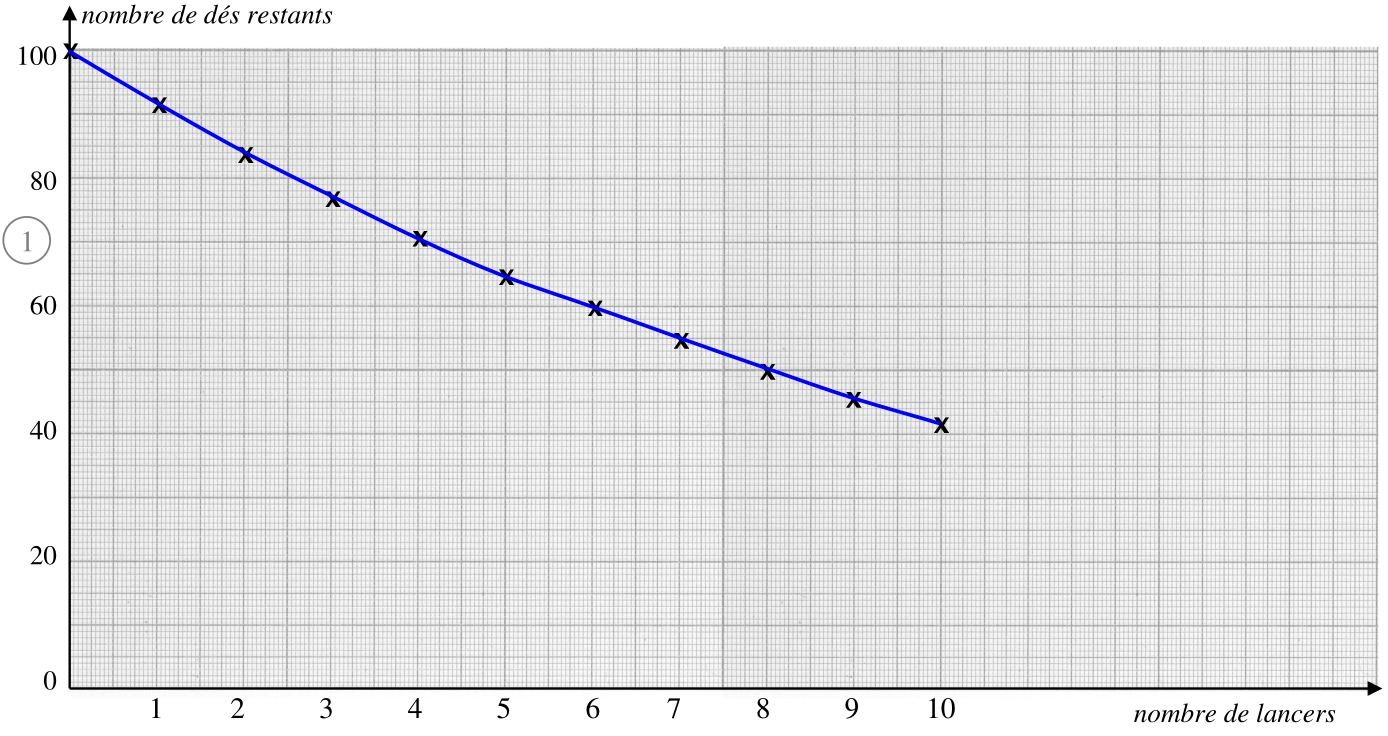
\includegraphics[width=0.7\textwidth]{images/physique_nucleaire/pn-003-000.png}
\caption{Loi de désintégration radioactive.}
\end{figure}

\begin{figure}[H]
\centering

\includegraphics[width=0.7\textwidth]{images/physique_nucleaire/pn-003-001.png}
\caption{Décroissance exponentielle du nombre de noyaux.}
\end{figure}

\begin{figure}[H]
\centering
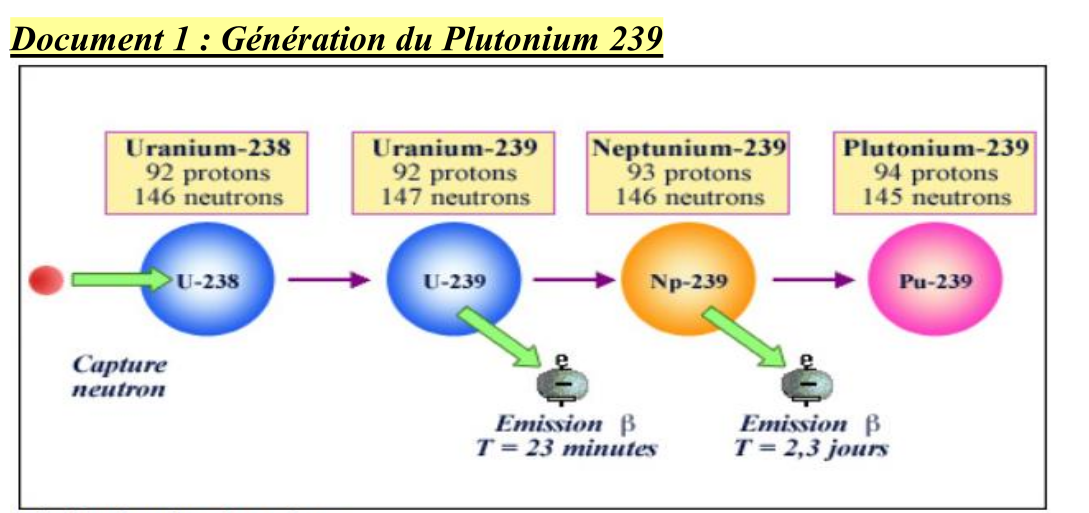
\includegraphics[width=0.7\textwidth]{images/physique_nucleaire/pn-012-002.png}
\caption{Fission nucléaire de l'uranium 235.}
\end{figure}

\begin{figure}[H]
\centering

\includegraphics[width=0.7\textwidth]{images/physique_nucleaire/pn-012-003.png}
\caption{Réaction en chaîne dans un réacteur nucléaire.}
\end{figure}

\ifdefined\inMainDoc\else\end{document}\fi
